84. \begin{figure}[ht!]
\center{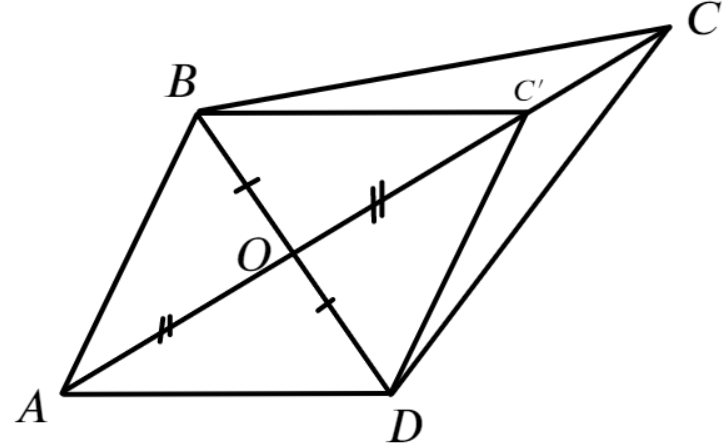
\includegraphics[scale=0.35]{g8-169.png}}
\end{figure}\\
Отложим на отрезке $OC$ точку $C'$ так, чтобы $AO=OC'$ (это можно сделать, так как $AO<OC$). Тогда в четырёхугольнике $ABC'D$ диагонали делятся точкой пересечения пополам, значит он является параллелограммом и $\angle BC'D=\angle BAD.$ Углы $BC'O$ и $DC'O$ являются внешними в треугольниках $BC'C$ и $DC'C,$ поэтому $\angle BAD=\angle BC'D=\angle BC'O+\angle DC'O=\angle C'BC+\angle C'CB+\angle C'DC+\angle C'CD=\angle BCD+\angle C'BC+\angle C'DC>\angle BCD,$ ч.т.д.\\
